\subsubsection{Encabezado de la sección ``Detalles de las campañas''}
Cuando el usuario entra a ver la información de una campaña, lo primero que puede ver es el encabezado de la página. En este encabezado se puede ver información básica de la campaña como su nombre, el logo y el banner, además, el usuario también podrá ver la cantidad de puntos que tiene en esa campaña.

Otro componente que podrá ver el usuario es uno llamado ``Breadcrumbs'' que básicamente es un pequeño menú de navegación que muestra toda la ruta de páginas que debió seguir el usuario para llegar a la sección donde se encuentra actualmente.

El encabezado se ve de la siguiente manera (Ver Figura 11):

    \begin{figure}[H]
        \begin{center}
            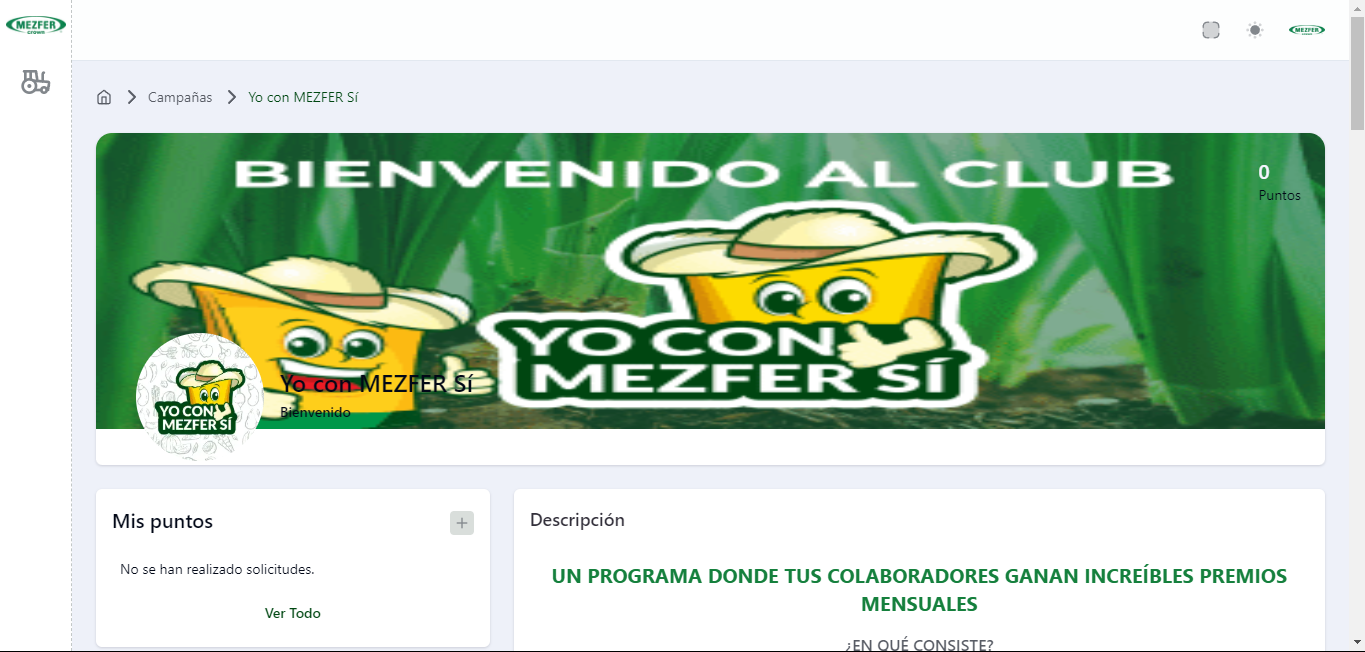
\includegraphics[scale=0.26]{img/actividades/detalles-campanias/encabezado.png}
            \caption{Encabezado de la sección.}
            \label{fig:encabezado}
        \end{center}
    \end{figure}